\documentclass[10pt,a4paper]{article}
\usepackage[utf8]{inputenc}
%\usepackage[bulgarian]{babel}
\usepackage{amsmath}
\usepackage{amsfonts}
\usepackage{amssymb}
\usepackage{graphicx}
\usepackage[left=2cm,right=2cm,top=2cm,bottom=2cm]{geometry}

\usepackage{listings}    
\lstset{language=R} 

\begin{document}
\title{R deltaScoring package description}
\author{Dimitar Atanasov\\ datanasov@nbu.bg}

\maketitle

\section{Instalation}

\section{Item responses}
The dihotomous item response (0/1) should be in a numeric array. For example 
\begin{lstlisting}
install.packages("random")  
library("random")

itemData<- randomNumbers(n = 5000,min = 0,max = 1,col = 20) 
 
\end{lstlisting}

\section{Estimating item delta}
Estimating the main item parameter {\bf delta}, reffered as $\delta$  in the refferences is estimated by a bootstrap procedure
\begin{lstlisting}
Itm<-dS.deltaBootstrap(itemData) 
\end{lstlisting}

The result is a list with {\bf delta} and {\bf conf} fields, containig delta values and their 90\% confidence interval respectivelly.
\begin{lstlisting}
> Itm$delta
      delta
 [1,] 0.492
 [2,] 0.500
 [3,] 0.508
 [4,] 0.544
 [5,] 0.464
 [6,] 0.504
 [7,] 0.496
 [8,] 0.508
 [9,] 0.516
 .
 .
 .
 
 > Itm$conf
        0.05   0.95
 [1,] 0.4400 0.5480
 [2,] 0.4480 0.5520
 [3,] 0.4560 0.5600
 [4,] 0.4920 0.5960
 [5,] 0.4120 0.5200
 .
 .
 .
\end{lstlisting}

\section{Person D-score}
Person D-score (see \cite{1}) is caclulated by the person response vector and the item deltas
\begin{lstlisting}
Dscores<-dS.personDscore(itemData,Itm$delta)

> Dscores
            [,1]
  [1,] 0.5521669
  [2,] 0.7018459
  [3,] 0.5565811
  [4,] 0.3976726
  [5,] 0.4069021
  [6,] 0.4434189
  [7,] 0.5425361
  [8,] 0.5052167
  .
  .
  .
\end{lstlisting}

\section{Fit RFM Model}
The RFM model defines the probability for corresct tem performace as 1,2 or 3 parametric function \cite{1}. The corresponding paramters ($b,s,c$) are estimated for any item in the test. The fitted {\tt parameters}, {\tt p-Values} and standard errors {\tt SE} are returned in the list {\tt Fit}.

\begin{lstlisting}
Fit<-dS.logitDeltaFit(itemData,Dscores)

Fit$parameters
Fit$pValues
Fit$SE
\end{lstlisting}

The default model is RFM2 with parameters $b$ and $s$ for the dificulty and shape of the ICC. If a diferent model is required, it can be changed trough the additional option parameter. For example, the following code fits the RFM3 model
\begin{lstlisting}
o <- dS.options()
o$model <- 3
Fit<-dS.logitDeltaFit(itemData,Dscores,o)
\end{lstlisting}

The plot of the ICC can be generated by the code bellow, there the items 3,5,7 will be ploted in the same plot with a corresponding legend.

\begin{lstlisting}
dS.logitDeltaPlot(Fit,items = c(3,5,7))
\end{lstlisting}

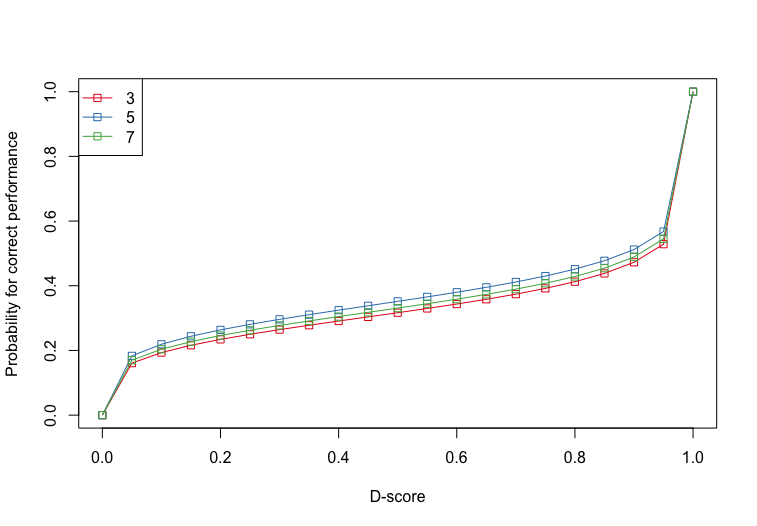
\includegraphics[scale=0.5]{icc.png}

\section{Equating}


\begin{thebibliography}{9}
\bibitem{1} Dimitrov, Dimiter. (2019). Modeling of Item Response Functions Under the D -Scoring Method. Educational and Psychological Measurement. 80. 001316441985417. 10.1177/0013164419854176. 
\end{thebibliography}
\end{document}